\documentclass[12pt,letterpaper]{article}
\usepackage[utf8]{inputenc}
\usepackage{amsmath}
\usepackage{amsfonts}
\usepackage{amssymb}
\usepackage[spanish]{babel}
\usepackage{amsmath}
\usepackage{amsfonts}
\usepackage{amssymb}
\usepackage{ragged2e}
\usepackage{graphicx}
\usepackage{fancyhdr}
\usepackage[lmargin=2.54cm, rmargin=2.54cm, top=2.54cm, bottom=2.54cm]{geometry}


\begin{document}
\begin{titlepage}
\begin{center}



{ \LARGE \textbf{ECUACIONES DIFERENCIALES}} \\
\vspace{0.5cm}
{\large \textbf{APLICACIONES DE LAS ECUACIONES DIFERENCIALES DE PRIMER ORDEN}} \\
\vspace{0.2cm}
{\normalsize \textbf{Trayectorias Ortogonales y Oblicuas}} \\
\begin{figure}[h]
\centering

\includegraphics[scale=0.5]{Logo Uni}
\end{figure}
\textbf{Presentado por:} Victor Manuel Ordoñez Delgado \par
\vspace{0.5cm}
\textbf{Docente:} Jonathan Collazos \par
\vspace{2cm}
\textbf{UNIVERSIDAD DEL CAUCA}\par
\vspace{0.5cm}
\textbf{FACULTAD DE INGENIERÍA CIVIL} \par
\vspace{0.5cm}
\textbf{INGENIERÍA CIVIL} \par
\vspace{0.5cm}
\textbf{Popayán, Cauca} \par
\vspace{0.5cm}
2022 \par

\end{center}
\end{titlepage}
\begin{titlepage}



\section{\Large APLICACIONES DE LAS ECUACIONES DIFERENCIALES DE PRIMER ORDEN}

\vspace{1cm}

\subsection{\normalsize { INTRODUCCIÓN}}
\justify
El estudio de las ecuaciones diferenciales lleva consigo gran serie de aplicaciones y en diferentes campos, es necesario entonces crear modelos matematicos que permitan dar solución a un problema o necesidad, de ahí la importancia del análisis y la investigación de las ecuaciones diferenciales. 

Como una de las aplicaciones más importantes y llamativas se estudiarán las aplicaciones geométricas, es decir, trayectorias ortogonales y oblicuas. Esto permitirá encontrar curvas que intersecan curvas dadas ya sea en ángulo recto o no; si el respectivo ángulo es recto, a las nuevas curvas se les conoce como trayectorias ortogonales a las curvas dadas; de lo contrario serán trayectorias oblicuas o isogonales a las curvas dadas.

Las trayectorias ortogonales y oblicuas son de gran interés en la ingeniería, geometría, física y en algunas situaciones de matemática aplicada. Mencionando algunos ejemplos en particular, se pueden las aplicaciones en los planos topográficos y geológicos, donde se tienen información de curvas de nivel y estas son proyectadas de manera perpedincular en el plano. En la física se pueden ver en los campos magnéticos, eléctricos, conducción de calor, dinámica de fluidos entre otros.

En ese sentido, el presente muestra uno de los métodos para obtener tanto trayectorias ortogonales como oblicuas a una familia de curvas dadas, y asi mismo se indican algunos ejemplos de las aplicaciones más importantes.



\end{titlepage}

\begin{titlepage}
\subsection{FAMILIA DE CURVAS}
\begin{flushleft}


La solución general de una ecuación diferencial de primer orden contiene generalmente una costante arbitraria llamada parámetro. Cuando a este parámetro se le asignan valores, obtenemos una familia uniparamétrica de curvas. Cada una de estas curvas es solución de la ecuación diferencial dada y todas juntas constituyen la solución general.

\vspace{0.5cm}
Si para cada valor fijo de $ c $ la ecuación:

\vspace{0.3cm}
\centering
$F(x, y, c) = 0$
\vspace{0.5 cm}

\end{flushleft}

\begin{flushleft}
Representa una curva en el plano $xy$ y si para $c$ variable representa uan familia de curvas, entonces la totalidad de estas curvas se le llama familia de curvas con un parámetro, y a $c$  se le llama parámetro de familias. \\
    
Es posible obtener muchas familias con un parámetro a partir de la solución general de una ecuación diferencial, la cual contiene un parámetro arbitrario $c$ en consecuencia, dada una familia de curvas, el primer paso del método que se presenta es aplicar derivación implicita y se resolver la ecuación diferencial que permita hallar la familia de trayectorias.

\end{flushleft}
\vspace{0.3 cm}
\subsection{APLICACIONES GEOMÉTRICAS}
\vspace{0.1cm}
\subsubsection{TRAYECTORIAS ORTOGONALES Y TRAYECTORIAS OBLICUAS}

\begin{flushleft}

\textbf{Definición:} Sean $f(x,y,c) = 0$ y $g (x,y,k) = 0$ dos familias de curvas y sea $\theta$ el ángulo que forman las rectas tangentes a cada par de curvas (de cada familia) en cada punto de intersección.
\begin{itemize}
\item[i)] Si $\theta = \frac{\pi}{2},$ entonces $g(x,y,k) = 0$ es la familia de \textbf{trayectorias ortogonales} de $f(x,y,c) = 0$ 

\item[ii)] Si $ 0 < \theta < \frac{\pi}{2},$ entonces se dice que $g(x,y,k) = 0$ es la familia de \textbf{trayectorias oblicuas} a $\theta$, de la familia $f(x,y,c) = 0$ 

\end{itemize}
\begin{center}

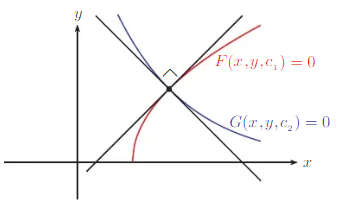
\includegraphics[scale=1]{Figura Trayec Ortogona}

Figura 1: Trayectorias Ortogonales
\end{center}
\end{flushleft}

\end{titlepage}
\begin{titlepage}


\begin{center}

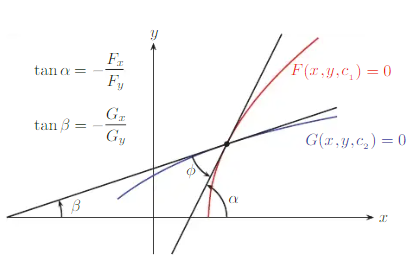
\includegraphics[scale=1]{Figura Trayec Oblicuas}

Figura 2: Trayectorias Oblicuas
\end{center}

\begin{center}

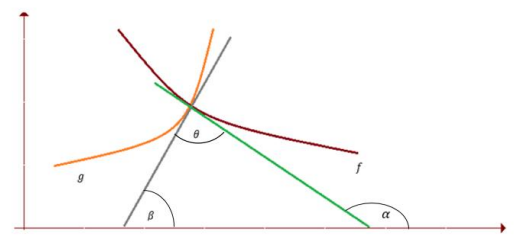
\includegraphics[scale=0.9]{Fig Funciones f y g}

Figura 3: Funciones f y g 
\end{center}
\begin{flushleft}

\textbf{De acuerdo con la figura 3 se puede notar que: } \\
\begin{itemize}
\item[-] Las funciones $f$ y $g$, representan respectivamente una curva de cada familia, y $P$ es el punto de intersección de dichas curvas.

\item[-] $\alpha$ es el ángulo (no negativo) que forma la recta tangente a $f$ en el punto $P$, $\beta$ es el ángulo (no negativo) que forma la recta tangente a $g$ en el punto $P$ y $\theta$ es el ángulo que forman las rectas tangentes, en el punto $P$.
\item[-] Como $\alpha$ es un ángulo exterior del triángulo determinado por las rectas tangentes y el eje $x$, entonces \\

\centering
\begin{eqnarray}
\alpha = \beta + \theta \Leftrightarrow \theta = \alpha - \beta
\end{eqnarray}

\item[-] La pendiente de cada una de las rectas tangentes a cada una de las curvas $f$ y $g$ en el punto $P$ está dada por: 

\begin{eqnarray}
\tan \alpha = f'(x) \hspace{0.5cm} y \hspace{0.5cm} \tan \beta = g'(x)
\end{eqnarray}

\begin{flushleft}
\item[-] Si las rectas tangentes son perpendiculares, entonces se cumplen que:
\begin{eqnarray}
f'(x)g'(x) = -1
\end{eqnarray}
\end{flushleft}

\begin{flushleft}
La ecuación (3) es una ecuación diferencial y su solución permite establecer la familia de trayectorias ortogonales a una familia de curvas dada.
\end{flushleft}
\begin{flushleft}
\item[-] Si $ 0 < \theta < \frac{\pi}{2}$, entonces en (1) tenemos que:
\begin{eqnarray}
\tan \theta = \tan (\alpha - \beta)
\end{eqnarray}
\end{flushleft}

\begin{flushleft}
Por identidades trigonométricas se tiene que
\begin{eqnarray}
\tan \theta = \tan (\alpha - \beta) = \frac{\tan \alpha - \tan \beta}{1 + \tan \alpha \tan \beta}
\end{eqnarray}
Sustituyendo (2) en (5) se obtiene:
\begin{eqnarray}
\tan \theta = \frac{f'(x)- g'(x)}{1 + f'(x)g'(x)}
\end{eqnarray} 
La ecuación (6) es una ecuación diferencial y su solución permite establecer la familia de trayectorias oblicuas a $\theta$, de una familia de curvas dada.
\end{flushleft} 
\end{itemize}
\end{flushleft}

\subsubsection{PROCEDIMIENTO PARA HALLAR TRAYECTORIAS ORTOGONALES}
\begin{flushleft}
Supongamos que la ecuación que describe una familia de curvas está dada por:
\begin{equation} \tag{1} \label{ecu1}
f(x,y) = C
\end{equation}
Para establecer la familia de trayectorias ortogonales a dicha familia se procede asi:\\
\vspace{0.6cm}
Paso 1: Llevar la ecuación que describe a la familia dada, a la forma \eqref{ecu1}, siempre que sea necesario.\\
\vspace{0.6cm}
Paso 2: Derivar respecto a x en \eqref{ecu1} y obtener $f'(x)$
\begin{equation*}
\dfrac{d}{dx} [f(x,y)] = \dfrac{d}{dx}[C]
\end{equation*}
\end{flushleft}
\end{titlepage}

\begin{titlepage}
\begin{flushleft}
Paso 3: Plantear y resolver la ecuación diferencial que modela el problema 
\begin{equation} \tag{2} \label{ecu2}
f'(x)y' = -1
\end{equation}
Donde $y'$ \hspace{0.02cm} = \hspace{0.02cm} $g'(x)$, siendo g una curva en la familia de trayectorias ortogonales. \\
\vspace{0.4 cm}
Si la solución general de \eqref{ecu2} es $g(x,y) = K$, esta corresponde a la familia de trayectorias ortogonales de la familia $f(x,y,C) = 0$.\\

\vspace{0.5cm}
\textbf{Ejemplo 1:}\\
\vspace{0.5cm}
Hallar la familia de trayectorias ortogonales de la familia
\begin{equation} \tag{1} \label{ec1}
y^{2} = cx^{3}
\end{equation}

\textbf{Solución:} \\
\vspace{0.5cm}
 Paso 1: Si x $\neq$ 0, entonces de \eqref{ec1} se tiene que:
\begin{equation} \tag{2} \label{ec2}
\frac{y^{2}}{x^{3}} = c
\end{equation}

Paso 2: Aplicando derivación implicita en \eqref{ec2} se tiene:
\begin{equation*} 
\dfrac{d}{dx} [y^{2}x^{-3}] = \dfrac{d}{dx} [c],\hspace{0.2cm} y = f(x)
\end{equation*}
\begin{equation} \tag{3} \label{ec3}
x^{-3}(2yy') + y^{2}(-3x^{-4}) = 0
\end{equation}
Luego,\\
\begin{equation} \tag{4} \label{ec4}
y' = f'(x) = \dfrac{3y}{2x}
\end{equation}
Paso 3: Describamos y resolvamos la ecuación diferencial que permite hallar la familia de trayectorias ortogonales, representadas por g.
\begin{equation*}
f'(x)g'(x) = -1 \Leftrightarrow \dfrac{3y}{2x}g'(x)=-1 \Leftrightarrow \dfrac{3y}{2x} \frac{dy}{dx} \tag {edvs}
\end{equation*}
\begin{equation*}
ydy = - \dfrac{2}{3} xdx \Leftrightarrow \int ydy = - \int \frac{2}{3} xdx \Leftrightarrow \frac{y^{2}}{2} = -\dfrac{x^{2}}{3} + k
\end{equation*}
\begin{equation} \tag{5} \label{ec5}
\frac{y^{2}}{2} + \frac{x^{2}}{3} = k 
\end{equation}
\textbf{Respuesta:}\\
\vspace{0.5cm}
Si $k > 0$, enotnces la ecuación \eqref{ec5} representa a la familia de trayectorias ortogonales (elipses con centro en el origen de coordenadas) a la familia dada.
\end{flushleft}
\end{titlepage}

\begin{titlepage}
\begin{flushleft}
\textbf{Ejercicio 1:} \\
\vspace{0.5cm}
Hallar la familia de trayectorias ortogonales de la siguiente familia. 
\begin{equation} \tag{1} \label{ecua1}
x^{2} + y^{2} = cx
\end{equation}
\textbf{Solución:} \\
\vspace{0.5cm}
 Paso 1: Si x $\neq$ 0, entonces de \eqref{ecua1} se tiene que:
\begin{equation} \tag{2} \label{ecua2}
\frac{x^{2}}{x} + \frac{y^{2}}{x} = c \Leftrightarrow x + \frac{y^{2}}{x} = c
\end{equation}
Paso 2: Aplicando derivación implicita en \eqref{ecua2} se tiene:
\begin{equation*} 
\dfrac{d}{dx} [x] + \dfrac{d}{dx} [\frac{y^{2}}{x}] = \dfrac{d}{dx} [c],\hspace{0.2cm} y = f(x)
\end{equation*}
\begin{equation*} 
1 + \frac{2yy'x - y^{2}}{x^{2}} = 0
\end{equation*}
\begin{equation*} 
 \frac{2yy'x - y^{2}}{x^{2}} = -1
\end{equation*}
\begin{equation} \tag{3} \label{ecua3}
 2yy'x - y^{2} = -x^{2}
\end{equation}
Luego,\\
\begin{equation} \tag{4} \label{ecua4}
y' = f'(x) = \dfrac{-x^{2} + y^{2}}{2xy}
\end{equation}
Paso 3: Describamos y resolvamos la ecuación diferencial que permite hallar la familia de trayectorias ortogonales, representadas por g.
\begin{equation*}
f'(x)g'(x) = -1 \Leftrightarrow \dfrac{-x^{2} + y^{2}}{2xy} g'(x)=-1 \Leftrightarrow \dfrac{-x^{2} + y^{2}}{2xy} \frac{dy}{dx} = -1 \tag{edh}
\end{equation*}
\begin{equation} \tag{5} \label{ecua5}
\frac{dy}{dx} = \dfrac{2xy}{x^{2} - y^{2}}
\end{equation}
Paso 4: Rsolviendo la ecuación diferencial homogenea obtenida se tiene:
\begin{equation}  \tag{6} \label{ecua6}
\frac{dy}{dx} = h(x,y)= \dfrac{2xy}{x^{2} - y^{2}}
\end{equation}
Haciendo cambio de variable:
\begin{equation}\tag{a} \label{ecuaa}
y = zx
\end{equation}
\begin{equation}\tag{b} \label{ecuab}
\frac{dy}{dx} = z + x \frac{dz}{dx}
\end{equation}
Sustituyendo \eqref{ecuaa} y \eqref{ecuab} en \eqref{ecua6} se obtiene:
\begin{equation*} \tag{edvs}
z + x \frac{dz}{dx} = \frac{2zx*x}{x^{2}- (zx)^{2}}
\end{equation*}
\end{flushleft}
\end{titlepage}
\begin{titlepage}
\begin{flushleft}

Se resuelve la ecuación diferencial de variables separables obtnida en el paso anterior:
\begin{equation*} 
z + x \frac{dz}{dx} = \frac{2zx^{2}}{x^{2}- z^{2}x^{2}}
\end{equation*}
\begin{equation*} 
z + x \frac{dz}{dx} = \frac{2z}{(1- z^{2})}
\end{equation*}
\begin{equation*} 
x \frac{dz}{dx} = \frac{2z}{(1- z^{2})} - z
\end{equation*}
\begin{equation*} 
x{dz} = \frac{z + z^{3}}{1- z^{2}} dx 
\end{equation*}
\begin{equation*} 
\int\frac{1- z^{2}}{z + z^{3}} dz = \int \frac{dx}{x} 
\end{equation*}
Resolviendo la integral del lado izquierdo:
\begin{equation*} 
\int\frac{1- z^{2}}{z + z^{3}} dz = \int\frac{1+z^{2} - z^{2} - z^{2}}{z + z^{3}} dz
\end{equation*}

\begin{equation*} 
 \hspace{1.8cm}= \int\frac{(1+z^{2}) - 2z^{2}}{z (1+ z^{2})} dz
\end{equation*}

\begin{equation*} 
 \hspace{2.5cm}= \int\frac{1}{z} dz - \int\frac{2z}{(1+ z^{2})} dz
\end{equation*}

\begin{equation*} 
\int\frac{1- z^{2}}{z + z^{3}} dz = \ln(z)- \ln(1+ z^{2}) + A
\end{equation*}

Resolviendo la integral del lado derecho:
\begin{equation*} 
\int \frac{1}{x} \,dx = \ln(x) + B
\end{equation*}

Luego,
\begin{equation} \tag{7} \label{ecua7}
\ln(\frac{y}{x})- \ln(1 + \frac{y^{2}}{x^{2}}) = \ln(x) + k
\end{equation}

\textbf{Respuesta:}\\
\vspace{0.5cm}
Para todo $k \in \mathbb R $, la ecuación \eqref{ecua7} representa la familia de trayectorias ortogonales  a la familia dada.
\end{flushleft}
\end{titlepage}

\begin{titlepage}
\begin{flushleft}
\subsubsection{PROCEDIMIENTO PARA HALLAR TRAYECTORIAS OBLICUAS} 

Sea,
\begin{equation} \tag{1} \label{for1}
f(x,y) = C
\end{equation}

Para establecer la familia de trayectorias oblicuas al ángulo $\theta$, de dicha familia, se sigue como se indica a continuación:

\vspace{0.6cm}
Paso 1: Llevar la ecuación que decribe a la familia dada, a la forma \eqref{for1}, siempre que sea necesario.
\vspace{0.6cm}

Paso 2: Derivar respecto a $x$ en \eqref{for1} para obtener $f'(x)$
\begin{equation*}
\dfrac{d}{dx} [f(x,y)] = \dfrac{d}{dx}[C]
\end{equation*}

Paso 3: Plantear y resolver la ecuación diferencial que modela el problema.
\begin{equation} \tag{2} \label{for2}
\tan \theta = \frac{f'(x) - y'}{1+ f'(x)y'}
\end{equation}

Donde $y' = g'(x)$, siendo g una curva en la familia de trayectorias oblicuas al ángulo $\theta$.\\
\vspace{0.5 cm}
Si la solución general de \eqref{for2} es $g(x,y) = K$, esta corresponde a la familia de trayectorias oblicuas al ángulo $\theta$, de la familia $f(x,y,C) = 0$
\vspace{0.5cm}

\textbf{Ejemplo 2:}\\
\vspace{0.5cm}
Hallar las trayectorias oblicuas a $\theta$ $ = \frac{\pi}{4}$ para la familia $ y( x+C ) = 1 $ 

\textbf{Solución:} \\
\vspace{0.5cm}
Paso 1: Si y $\neq$ 0, entonces: 

\begin{equation} \tag{1} \label{forma1}
y( x+C ) = 1 \Leftrightarrow x + C = \frac{1}{y}
\end{equation}
Luego, 
\begin{equation} \tag{2} \label{forma2}
y^{-1} - x = C 
\end{equation}

Paso 2: Aplicando derivación implícita en \eqref{forma2} se tiene que:
\begin{equation} \tag{3} \label{forma3}
-y^{-2}y' - 1 = 0 
\end{equation}
Asi se obtiene:
\begin{equation*} 
f'(x) = y' = -y^{2} 
\end{equation*}
Paso 3: Planteamiento y solución diferencial que describe el problema:
\begin{equation} \tag{4} \label{forma4}
\tan \theta = \frac{f'(x) - y'}{1+ f'(x)y'} \Leftrightarrow \tan \frac{\pi}{4} = \frac{ -y^{2} - g'(x)}{1+ (-y^{2})g'(x)}
\end{equation}
Donde $g$ representa la familia de trayectorias oblicuas.
\end{flushleft}
\end{titlepage}

\begin{titlepage}
\begin{flushleft}
De la ecuación \eqref{forma4} se tiene que:
\begin{equation*} 
1 = \frac{ y^{2} + g'(x)}{y^{2}g'(x) - 1} \Leftrightarrow y^{2}g'(x) -1 = y^{2} + g'(x)
\end{equation*}
\begin{equation} \tag{5} \label{forma5}
g'(x) = \frac{dy}{dx} = \frac{y^{2} + 1} {y^{2} - 1} 
\end{equation}

La ecuación \eqref{forma5} es una ecuación diferencial de variables separables y se procede a resolver:
\begin{equation*}
\frac{y^{2} - 1}{y^{2} + 1}dy = dx \Leftrightarrow (1 - \frac{2}{y^{2}+1})dy = dx
\end{equation*}
\begin{equation*}
\int (1 - \frac{2}{y^{2}+1})dy = \int dx
\end{equation*}	
\begin{equation*}
y - 2 \arctan y \hspace{0.5 cm} = \hspace{0.5 cm} x + K
\end{equation*}
	
\textbf{Respuesta:}\\
\vspace{0.5cm}
$\forall$ $k \in \mathbb R $, la familia de trayectorias oblicuas $ \theta = \frac{\pi}{4}$ está representada por la ecuación:
\begin{equation*}
y - x - 2 \arctan y \hspace{0.3 cm} = \hspace{0.3 cm} K
\end{equation*}

\textbf{Ejercicio 2:} \\
\vspace{0.5cm}
Hallar las trayectorias oblicuas a $ \frac{\pi}{6}$ para la familia: 
\begin{equation} \tag{1} \label{met1}
y = ce^{2x}
\end{equation}

\textbf{Solución:} \\
\vspace{0.5cm}
 Paso 1: De \eqref{met1} se tiene que:
\begin{equation} \tag{2} \label{met2}
\frac{y}{e^{2x}}  = c \Leftrightarrow ye^{-2x} = c
\end{equation}
Paso 2: Aplicando derivación implicita en \eqref{met2} se tiene:
\begin{equation} \tag{3} \label{met3}
-2ye^{-2x} + e^{-2x}y' = 0
\end{equation}
\begin{equation*} 
y' = \frac{2ye^{-2x}}{e^{-2x}}
\end{equation*}
\begin{equation*} 
y' = 2y
\end{equation*}
Donde se tiene que $f'(x) = y' = 2y $

\vspace{0.3cm}
Paso 3: Planteamineto y solución diferencial que permita hallar la familia de trayectorias oblicuas.

\begin{equation} \tag{4} \label{met4}
\tan \theta = \frac{f'(x) - y'}{1+ f'(x)y'} \Leftrightarrow \tan \frac{\pi}{6} = \frac{ 2y - g'(x)}{1+ 2yg'(x)}
\end{equation}

\end{flushleft}
\end{titlepage}

\begin{titlepage}
\begin{flushleft}

Donde $g$ representa la familia de trayectorias oblicuas a $\frac{\pi}{6}$.

\vspace{0.4cm}
De la ecuación \eqref{met4} se puede ver que:
\begin{equation*} 
\frac{1}{\sqrt{3}} = \frac{ 2y - g'(x)}{1+ 2yg'(x)}
\end{equation*}
\vspace{0.2cm}
\begin{equation*} 
1+ 2yg'(x) = 2y \sqrt{3} - \sqrt{3}g'(x)
\end{equation*}
\vspace{0.1cm}
\begin{equation*} 
2yg'(x)+ \sqrt{3}g'(x) = 2y \sqrt{3} - 1
\end{equation*}
\vspace{0.1cm}
\begin{equation} \tag{5} \label{met5}
g'(x) = \frac{dy}{dx} = \frac{2y \sqrt{3} - 1} {2y + \sqrt{3}} 
\end{equation}
Se resuelve la ecuación diferencial de variables separables obtenida en \eqref{met5}. 

\begin{equation*}
\frac{2y + \sqrt{3}}{2y \sqrt{3} - 1}dy = dx 
\end{equation*}
\vspace{0.1cm}
\begin{equation*}
\int \frac{2y + \sqrt{3}}{2y \sqrt{3} - 1}dy  = \int dx
\end{equation*}

\vspace{0.1cm}	
Resolviendo la integral del lado izquierdo:
\begin{equation*} 
\int \frac{2y + \sqrt{3}}{2y \sqrt{3} - 1}dy =
\end{equation*}
Haciendo una sustitución
\begin{equation*}
U = 2y \sqrt{3} - 1 \Leftrightarrow y = \frac{U + 1}{2\sqrt{3}} \Leftrightarrow dU = 2 \sqrt{3} dy
\end{equation*}
\begin{equation*} 
 \hspace{1cm}= \int \frac{2(\frac{U + 1}{2 \sqrt{3}})+ \sqrt{3}}{U}dy 
\end{equation*}

\begin{equation*} 
 \hspace{3.5cm}= \frac{1}{2 \sqrt{3}}( \int\frac{U + 1}{2 \sqrt{3}*U} dU + \int\frac{\sqrt{3}}{U}) dU
\end{equation*}
\begin{equation*} 
 \hspace{2.8cm}= \frac{1}{2 \sqrt{3}}((\frac{U}{2 \sqrt{3}} + \ln U ) + ( \ln U))
\end{equation*}
\begin{equation*} 
\int \frac{2y + \sqrt{3}}{2y \sqrt{3} - 1}dy \hspace{0.3 cm} = \hspace{0.3 cm} \frac{1}{6} 2y \sqrt{3} -1 + \frac{2}{3} \ln (2y \sqrt{3} - 1) + C_{1}
\end{equation*}

Resolviendo la integral del lado derecho:
\begin{equation*} 
\int \frac{1}{x} \,dx = \ln(x) + C_{2}
\end{equation*}

\end{flushleft}
\end{titlepage}

\begin{titlepage}
\begin{flushleft}

Luego,
\begin{equation} \tag{6} \label{met6}
\frac{1}{6} 2y \sqrt{3} -1 + \frac{2}{3} \ln (2y \sqrt{3} - 1) \hspace{0.3cm} = \hspace{0.3 cm} \ln(x) + k
\end{equation}

\textbf{Respuesta:}\\
\vspace{0.5cm}
Para cualquier valor de $k$, la familia de trayectorias oblicuas a $\frac{\pi}{6}$ está dada por:
\begin{equation*}
\frac{1}{6} 2y \sqrt{3} -1 + \frac{2}{3} \ln (2y \sqrt{3} - 1)\hspace{0.3 cm} = \hspace{0.3 cm} \ln(x) + k
\end{equation*}

\subsection{APLICACIÓN DE LAS TRAYECTORIAS ORTOGONALES}
\subsubsection{CURVAS EQUIPOTENCIALES}
Alrededor de una carga electrostática, si se desea ver en dos dimensiones, se pueden trazar curvas imaginarias que sean ortogonales a las líneas de fuerza de la carga y paralelas entre si, cada una de estas líneas, representará uns sucesión de puntos los cuales respecto a la carga, tengan el mismo potencial eléctrico, en tres dimensiones serían superficies equipotenciales.
\vspace{1cm}  


\centering
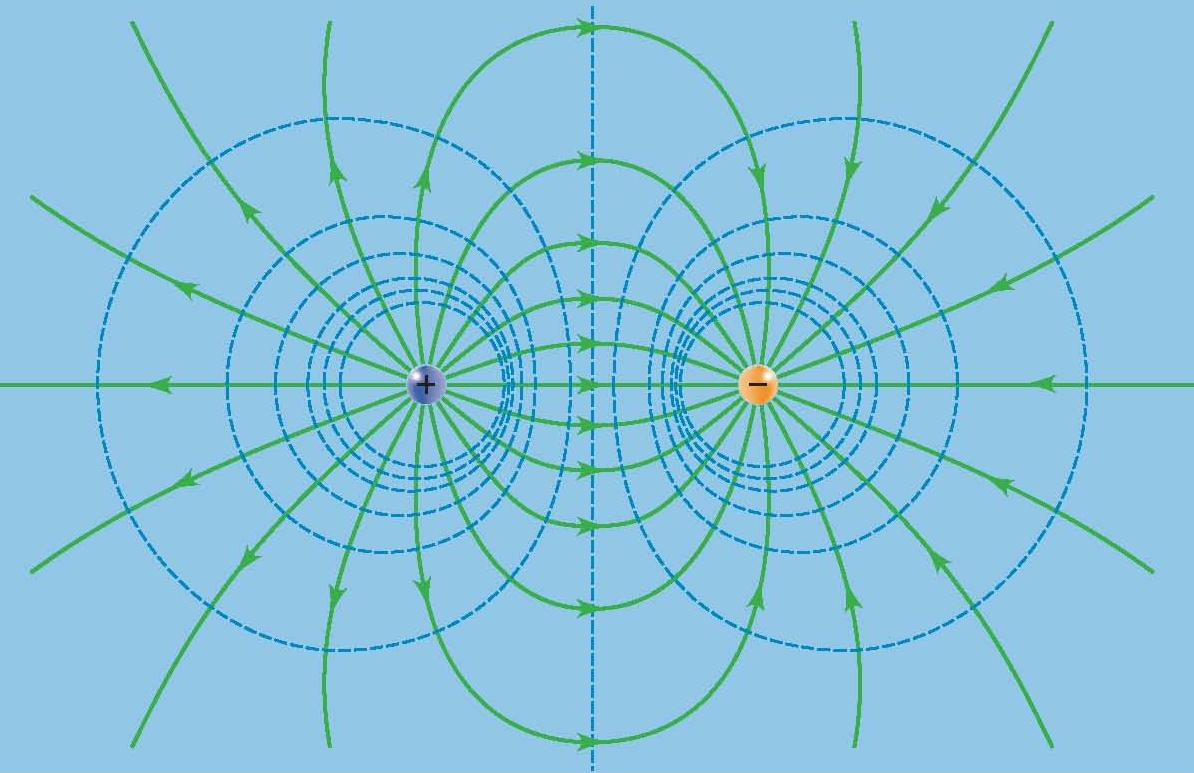
\includegraphics[scale=0.45]{Curvas equipotenciales}

Figura 4: Curvas equipotenciales


\end{flushleft}
\end{titlepage}

\begin{titlepage}
\begin{flushleft}

\subsubsection{CAMPOS MAGNÉTICOS}
Las líneas de fuerza que estan contenidas en un mapa mangético son circunferencias concéntricas, donde los centros de estas serán los diferentes puntos del conductor por donde circulan, los vectores del campo magnetico siempre serán tangentes a ella y estarán en planos perpendiculares a dicho conductor, esto nos dice que cumple con la principal característica de una trayectoria ortogonal.
\vspace{0.7cm}

\end{flushleft}
\centering
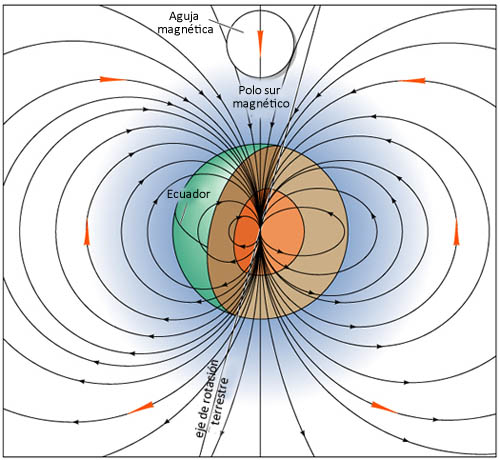
\includegraphics[scale=0.5]{Figura Campo magnetico}

Figura 5: Campo magnético

\begin{flushleft}


\subsubsection{LÍNEAS ISOTÉRMICAS}
La isoterma es un elemento y una herramienta que resulta fundamental a la hora de la medición de la temperatura de una zona determianada. En un plano cartográfico, la isoterma es una curva que une aquellos puntos que presentan las mismas temperaturas en una unidad de tiempo considerada.
\vspace{1cm}

\end{flushleft}
\end{titlepage}

\begin{titlepage}

\centering
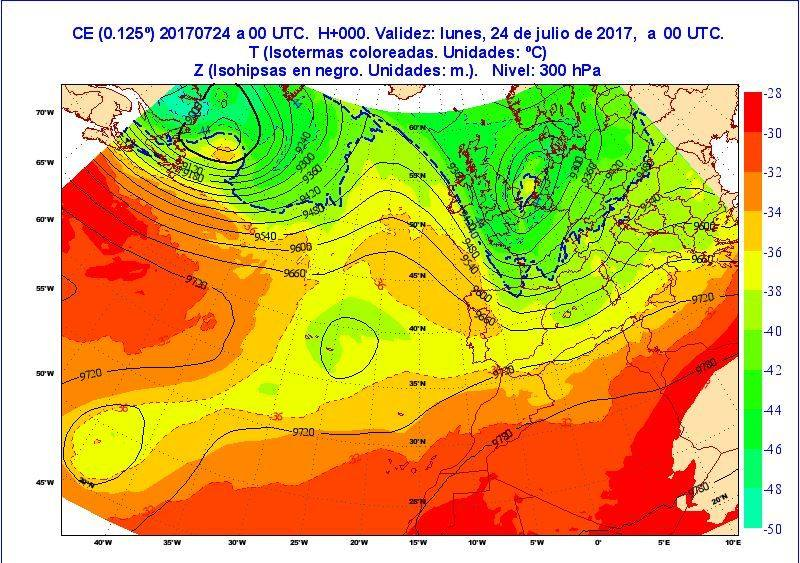
\includegraphics[scale=0.5]{Figura isotermicas}

Figura 6: Líneas Isotérmicas

\begin{flushleft}

\subsubsection{LÍNEAS ISOBÁRICAS}
Isobara o Isóbara es un isograma de presión, que consiste en una línea de igual o constante presión, en un gráfico, un trazado o mapa geológico y topográfico.
\end{flushleft}
\vspace{1cm}

\centering
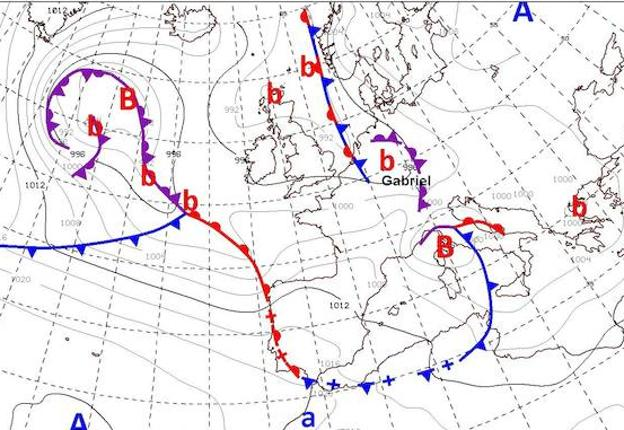
\includegraphics[scale=0.5]{Lineas isobaricas}

Figura 7: Líneas Isobáricas

\end{titlepage}


\begin{titlepage}
\centering
\textbf{CONCLUSIONES}
\vspace{0.3cm}

\begin{itemize}
\item[$\bullet$] Se pudo observar la manera de cómo encontrar familia de trayectorias ya sea ortogonales u oblicuas, haciendo uso del respectivo método explicado.\\

\item[$\bullet$] Fue posible analizar y estudiar una de las principales aplicaciones que tienen las ecuaciones diferenciales como lo son las trayectorias ortogonales y oblicuas.

\item[$\bullet$] Las aplicaciones de las trayectorias ortogonales y oblicuas, tienen interpretaciones inherentes al campo de estudio. Las aplicaciones que tienen mas relevancia como se pudo ver, están en la fisica como campos eléctricos y curvas equipotenciales.

\item[$\bullet$] Cuando se trata de aplicaciones en el campo de la ingeniería civil, el uso de las trayectorias ortogonales y oblicuas, están presentes en los panos topográficos y geológicos, ya que en estos aparecen curvas de nivel.

\item[$\bullet$] Es importante conocer y aplicar de buena manera las formas de resolver ecuaciones diferenciales de primer orden, ya que estos son indispensables al momento de tratar con trayectorias ortogonales y oblicuas.

\end{itemize}
\end{titlepage}

\begin{titlepage}
\centering
\textbf{BIBLIOGRAFÍA}
\vspace{0.3cm}

\begin{itemize}
\item[[ 1]] Mesa, F., Martínez Acosta, A., Gonzales Granada, J. R. (2012). Ecuaciones Diferenciales Ordinarias: una introducción. Pág: 44 (1.a ed.). Ecoe Ediciones.

\item[[ 2]] Carmona Jover, I., (1992). Ecuaciones Diferenciales Ordinarias. Pág: 129 (4.a ed.). editorial: Addison Wesley longman de México, S.A. de C.V.

\item[[ 3]] Gutierrez, J. A. (2019). ECUACIONES DIFERENCIALES DE TRAYECTORIAS ORTOGONALES E ISOGONALES. Scribd. Recuperado 25 de agosto de 2022, de https://es.scribd.com/document/475185949/ECUACIONES-DIFERENCIALES-DE-\\
TRAYECTORIAS-ORTOGONALES-E-ISOGONALES

\item[[ 4]] Terrios Guzman, L. M. CAPÍTULO 3: APLICAIONES DE LAS ECUACIONES DIFERENCIALES DE PRIMER ORDEN. Pág:40.

\item[[ 5]] KREYSZIG, E. (2003). MATEMÁTICAS AVANZADAS PARA INGENIERÍA (3.a ed., Vol. 1). Limusa, S.A. de C.V. 

\end{itemize}
\end{titlepage}

\end{document}
